\documentclass[border=6pt]{standalone}
\usepackage{fontspec}
\setmainfont{TeX Gyre Termes}
\usepackage{tikz}
\usetikzlibrary{arrows.meta,positioning,fit,backgrounds}
\definecolor{navy}{HTML}{16324F}
\definecolor{blue}{HTML}{2F6690}
\definecolor{green}{HTML}{3A7D44}
\definecolor{orange}{HTML}{D17A22}
\definecolor{red}{HTML}{A23E48}
\definecolor{lightblue}{HTML}{EAF3F8}
\definecolor{lightgreen}{HTML}{EAF5EC}
\definecolor{lightorange}{HTML}{FFF2DF}
\definecolor{lightred}{HTML}{FBEAEC}
\tikzset{
  box/.style={draw=navy, very thick, rounded corners=2pt, align=center, font=\small, inner sep=5pt, minimum height=0.9cm},
  data/.style={box, fill=lightblue, text width=2.25cm},
  calc/.style={box, fill=lightgreen, text width=2.25cm},
  agent/.style={box, fill=lightorange, text width=2.5cm},
  control/.style={box, fill=lightred, text width=2.5cm},
  arrow/.style={-{Latex[length=2.5mm]}, very thick, draw=navy},
  danger/.style={-{Latex[length=2.5mm]}, very thick, draw=red, dashed},
  label/.style={font=\scriptsize, align=center, fill=white, inner sep=2pt},
  participant/.style={box, fill=lightblue, text width=2.3cm, minimum height=0.75cm},
  zone/.style={box, minimum height=1.1cm, text width=4.1cm},
  smallbox/.style={box, font=\scriptsize, text width=3.5cm, minimum height=0.7cm}
}

\begin{document}
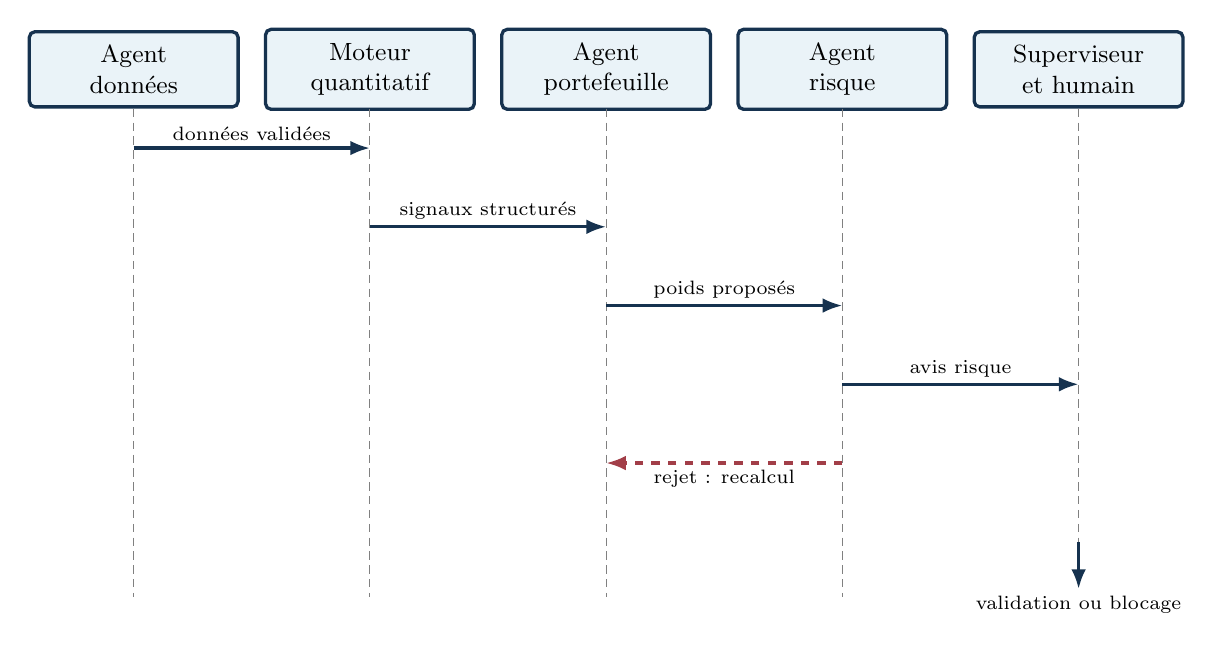
\begin{tikzpicture}[x=1cm,y=1cm]
\node[participant] (p1) at (0,0) {Agent\\données};
\node[participant] (p2) at (3,0) {Moteur\\quantitatif};
\node[participant] (p3) at (6,0) {Agent\\portefeuille};
\node[participant] (p4) at (9,0) {Agent\\risque};
\node[participant] (p5) at (12,0) {Superviseur\\et humain};
\foreach \x in {0,3,6,9,12} {\draw[densely dashed, gray] (\x,-0.5) -- (\x,-6.7);}
\draw[arrow] (0,-1) -- (3,-1) node[label,above,midway]{données validées};
\draw[arrow] (3,-2) -- (6,-2) node[label,above,midway]{signaux structurés};
\draw[arrow] (6,-3) -- (9,-3) node[label,above,midway]{poids proposés};
\draw[arrow] (9,-4) -- (12,-4) node[label,above,midway]{avis risque};
\draw[danger] (9,-5) -- (6,-5) node[label,below,midway]{rejet : recalcul};
\draw[arrow] (12,-6) -- (12,-6.6) node[label,below]{validation ou blocage};
\end{tikzpicture}
\end{document}
